\section{Introducere}
\subsection{Ce este Android?}

Android este un sistem de operare pentru dispozitive mobile bazat pe o versiune modificata a nucleului Linux.
Peste acest nucleu sunt adaugate librarii scrise in C si framework-ul pentru aplicatii creat pentru limbaje JVM.

\begin{figure}[H]
    \centering
    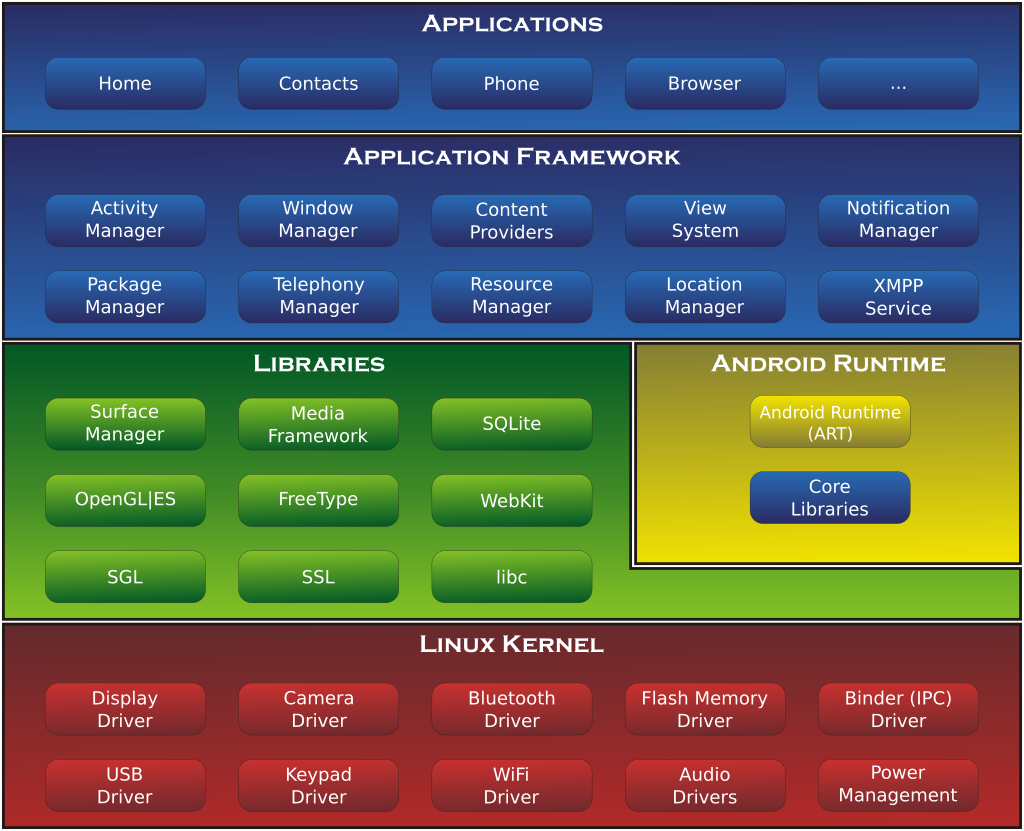
\includegraphics[width=0.7\linewidth]{figs/android_stack.png}
    \caption{Arhitectura sistemului de operare Android}
    \label{fig:android_stack}
\end{figure}

Este cel mai popular sistem de operare pentru dispozitive mobile, fiind fololsit de peste 75 \% din dispozitivele mobile.

\subsection{Capabilitatile de comunicare wireless ale dispozitivelor Android}
Datorita faptului ca Android este gandit in principal pentru dispozitive mobile, acesta ofera o serie de capabilitati de comunicare wireless, precum:
\begin{itemize}
    \item Wi-Fi
    \item Retele mobile
    \item Bluetooth
    \item NFC
\end{itemize}
Documentatia oficiala a Android ofera o serie de API-uri pentru a putea folosi aceste capabilitati in aplicatii: \url{https://developer.android.com/guide/topics/connectivity}
\subsection{Dezvoltarea aplicatiilor Android}
\subsubsection{Android Studio}
Mediul de dezvoltare oficial pentru Android este Android Studio, un IDE bazat pe IntelliJ IDEA, oferind o experienta similara.
Acesta vine cu o serie de facilitati pentru dezvoltarea aplicatiilor Android, precum un emulator pentru dispozitive mobile, un compilator si un depanator.
Poate fi descarcat gratuit de pe site-ul oficial: \url{https://developer.android.com/studio}
\subsubsection{Gradle}
Grade este un build system (asemantor cu Make sau Maven) care vine integrat in Android Studio.
\subsubsection{ADB}
ADB(Andorid Debug Bridge) este un tool care permite comunicarea cu dispozitivele Android, oferind o serie de comenzi pentru a instala aplicatii, a depana sau a face debugging.
\subsubsection{Logcat}
Logcat este un tool care permite vizualizarea log-urilor generate de aplicatii, fiind util pentru depanare.
\begin{figure}[H]
    \centering
    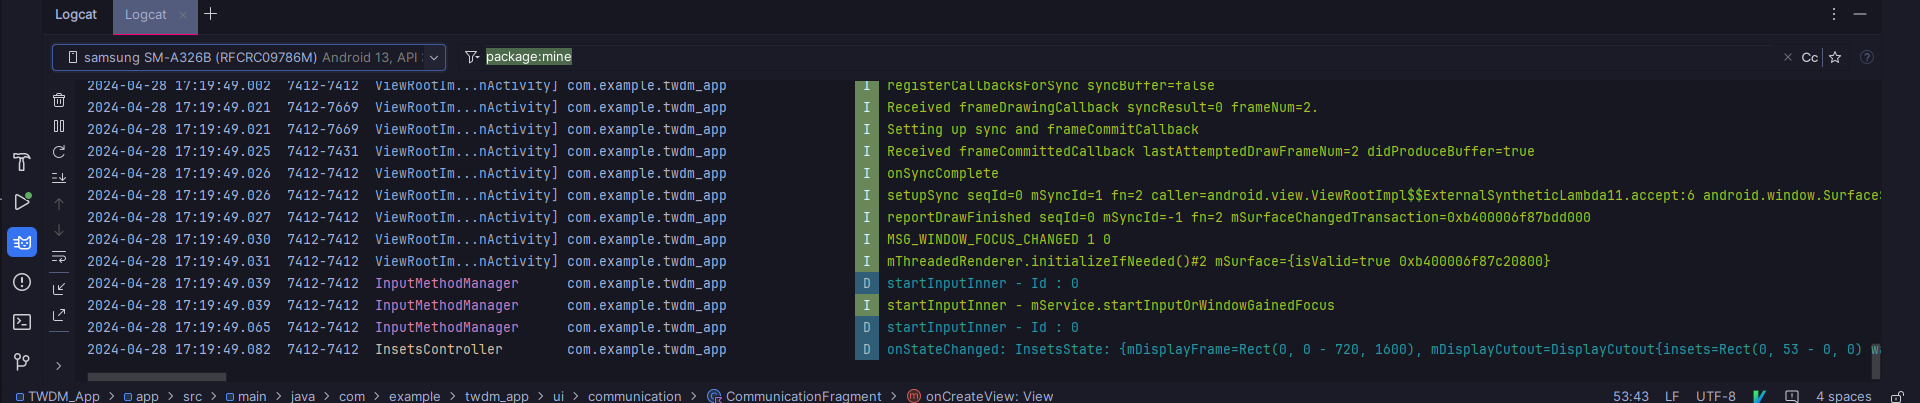
\includegraphics[width=0.7\linewidth]{figs/logcat_all.png}
    \caption{Logcat in Android Studio}
    \label{fig:logcat}
\end{figure}
Putem filtra log-urile dupa tag sau nivel de log, pentru a gasi mai usor informatiile de care avem nevoie.
\begin{figure}[H]
    \centering
    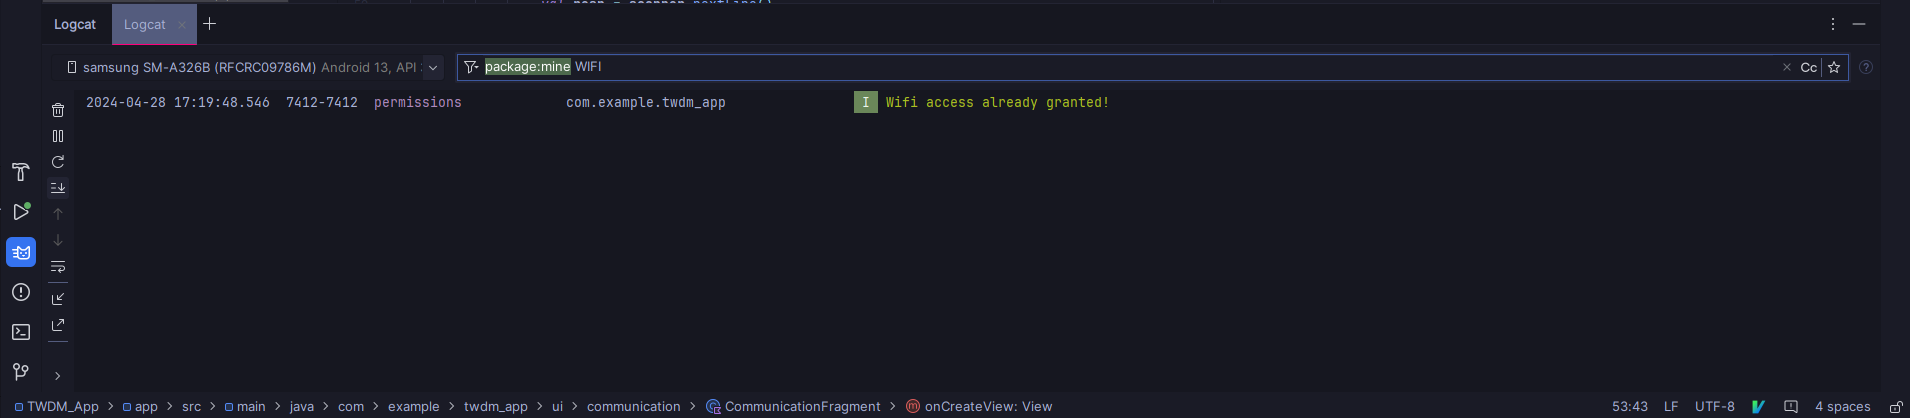
\includegraphics[width=0.7\linewidth]{figs/logcat_wifi.png}
    \caption{Filtrarea log-urilor in Android Studio}
    \label{fig:logcat_filter}
\end{figure}